\clearpage
\section{Experimental validation on a linear axis}
\label{sec:ExperimentalValidation}

The experimental validation reported in the previous \autoref{sec:shaker_test01} and \autoref{sec:shaker_test02} was carried out in a well-controlled environment with a shaker that was able to generate vibrations according to specific references. To further test the framework, a real-world application is considered in this section. The setup consists of a machine equipped with a linear axis, that is used to move a platform. On the moving platform the same accelerometer described in \autoref{tab:adxl335_specifications} has been attached using a custom 3D-printed fixture.

The test consists of defining a set of movements to be actuated by the platform, the accelerometer is used to capture the characteristics of each movement. As done previously, some movement profiles are used for training and others for testing. The position reference is shown in \autoref{fig:etel_profile}, and the parameters of the profiles are resumed in \autoref{tab:etel_profiles}.

\begin{figure}
    \centering
    \todo%\includegraphics{Images/etel/etel_profile.pdf}
    \caption{Position reference for the linear axis test}
    \label{fig:etel_profile}
\end{figure}

\begin{table}
    \centering
    \caption{Movement profiles of the linear axis}
    \label{tab:etel_profiles}
    \begin{tabular}{cccc} 
    \toprule
    \textbf{Profile N.} & \textbf{Speed} {[}$\text{m}\text{s}^{-1}$] & \textbf{Acceleration} {[}$\text{m}\text{s}^{-2}$] & \textbf{Jerk} {[}$\text{s}$] \\ 
    \hline
    1 & 0.8 & 6 & 0.02 \\
    2 & 0.4 & 3 & 0.02 \\
    3 & 0.4 & 6 & 0.02 \\
    4 & 0.6 & 8 & 0.02 \\
    \bottomrule
\end{tabular}
\end{table}

\subsection{Training}
To perform the training, a loop has been implemented on the \gls{pc} that manages the axis movements. The script cyclically actuates the axis to follow the reference profile and asks the microcontroller to start the acquisition of the accelerometer data at the beginning of the movement. The received \gls{glo:feature}s are then stored in a file, and the process is repeated for each profile. The sampling frequency of the microcontroller is 5kHz, for a total of 6000 samples each timeserie. 

Although not useful for the training, the microcontroller has been set not only to transmit the \gls{glo:feature}s to the \gls{pc} but also the time-series, for visualization purposes. The time-series of the training set are shown in \autoref{fig:axis_timeseries}, and the \gls{glo:feature}s are shown in \autoref{fig:axis_features}.

In the time-series set it is possible to see some outliers, for example, there is a record in which profile 1 started being actuated by the axis with a delay \gls{wrt} the others. Profile 4, instead, has some outliers due to the axis sometimes overshooting the reference position. These outliers are caused by the axis control, and the investigation about why it happens is out of the scope of this work. 

The training set contains 100 \gls{glo:snap}s for each profile, for a total of 400 \gls{glo:snap}s. The K-means model is then trained for $n=5$ \gls{glo:clust}s, according to the silhouette criterion.

As done previously, the training is performed with the user confirming the correct number of \gls{glo:clust}s. And updating the model into the microcontroller.

\begin{figure}
    \centering
    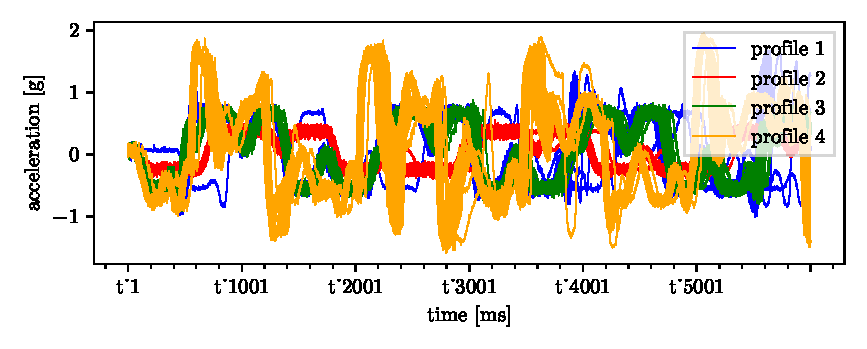
\includegraphics{images/LinearMotor/Timeseries.pdf}
    \caption{Timeseries of the training set}
    \label{fig:axis_timeseries}
\end{figure}


\begin{figure}
    \centering
    \includegraphics[width=\textwidth]{images/LinearMotor/Features.pdf}
    \caption{\gls{glo:feature}s of the training set}
    \label{fig:axis_features}
\end{figure}

\begin{figure}
    \centering
    \includegraphics{images/LinearMotor/Scatter.pdf}
    \caption{Visualization of the separation between profiles in the \gls{glo:feature} space}
    \label{fig:axis_scatter}
\end{figure}


\subsection{Testing on a known profile}
The microcontroller is then set in \emph{evaluate} mode and the \gls{nd} is performed on a loop that repeats the movement of profile 2. The result of this first model (Model 1) is shown in \autoref{fig:axis_testing}. We can see that the model immediately falsely detects a novelty, despite profile 2 being part of the training set. The figure also shows a clearer view of the evolution of the novelty score, obtained by applying a moving average filter on the last 5 values of the novelty metric.

Let's investigate why this model gives almost all false positive results. Analyzing the \gls{glo:feature}s of the training set (\autoref{fig:axis_features}), we can see that the first \gls{glo:feature}s, up to $\approx 12$, are grouped by profile, but most of the remaining \gls{glo:feature}s are not, this arises the suspect that these \gls{glo:feature}s may not be significative of the movement, but maybe just representing noise. This is likely also because the necessary standardization procedure ensures that each \gls{glo:feature} will have unitary standard deviation, regardless of the magnitude of the \gls{glo:feature} itself \gls{wrt} the others. This may cause \quoted{noise} \gls{glo:feature}s to be amplified in the model. Moreover, it's clear that, being most of the \gls{glo:feature}s not significant, the model is not able to distinguish between the profiles.

In \autoref{fig:axis_scatter}, a better visualization of the problem is presented. Features 5 and 6 are significative of the specific movement as we can see in the scatter plot, because the data points are grouped by profile. Features 25 and 26, instead, are not significative, as the data points are not grouped by profile.



\begin{figure}
    \centering
    \includegraphics[angle=-90,origin=c]{images/LinearMotor/Testing.pdf}
    \caption{Novelty detection on profile 2.}
    \label{fig:axis_testing}
\end{figure}
\clearpage


\subsection{Feature scaling}
To address the problem of the non-significative \gls{glo:feature}s, a \gls{glo:feature} scaling method is proposed. The idea is to scale the \gls{glo:feature}s in such a way that the most significant \gls{glo:feature}s will have a higher weight in the model. To do that, a naive approach could be to visually select the important \gls{glo:feature}s (by eye it's evident that are the first few) and apply a small scaling factor to the others. 

This approach goes against the principle of the framework being fully automatic to train. To address this problem, an unsupervised and automatic method is proposed. The idea is to scale the \gls{glo:feature}s in such a way that the most significant \gls{glo:feature}s will have a higher weight in the model. To do that, it's possible to exploit the fact that, at this point, the K-means model is already trained and the training procedure provided labels for the dataset. It's now possible to apply a \emph{supervised} \gls{ml} algorithm in a way that is transparent to the user, so the whole procedure remains \emph{unsupervised}.

The framework is then extended to include the possibility of applying \gls{glo:feature} scaling. The two possibilities are to use the Random Forest classifier or the SelectKBest algorithm to provide the weights. Since this scaling will affect also future \gls{glo:snap}s, a new train of the \gls{mla} is necessary. The new model is then trained with the same training set but with the scaled \gls{glo:feature}s. This approach is illustrated in \autoref{fig:scalingprocedure}.

\begin{figure}[h!]
    \centering
    \includegraphics{images/LinearMotor/Feat_scaling.pdf}
    \caption{Feature scaling procedure.}
    \label{fig:scalingprocedure}
\end{figure}

This scaling technique is used with several configurations for both scaling the \gls{glo:feature} and reducing the number of \gls{glo:feature}s, by discarding the unnecessary ones. The settings of each tuned model are resumed in \autoref{tab:axis_models}. These models are described later in this section.

\begin{table}
    \centering
    \caption{Tuned embedded models parameters}
    \label{tab:axis_models}
    \resizebox{\linewidth}{!}{%
    \begin{tabular}{ccccccccc} 
    \toprule
    \multirow{2}{*}{\textbf{Model}} & \multicolumn{2}{c}{\textbf{Feature Scaling}} & \multirow{2}{*}{\begin{tabular}[c]{@{}c@{}}\textbf{Feature}\\\textbf{Subset}\end{tabular}} & \multicolumn{4}{c}{\begin{tabular}[c]{@{}c@{}}\textbf{Training Snapshots}\\(per each profile)\\\end{tabular}} & \multirow{2}{*}{\begin{tabular}[c]{@{}c@{}}\textbf{N of}\\\textbf{\gls{glo:clust}s}\end{tabular}} \\
     & SelectKBest & Random Forest &  & 1 & 2 & 3 & 4 &  \\ 
    \hline
    Model 1 &  &  &  & 100 & 100 & 100 & 100 & 5 \\
    Model 2 &  & \checkmark &  & 100 & 100 & 100 & 100 & 3 \\
    Model 3 & \checkmark &  &  & 100 & 100 & 100 & 100 & 3 \\
    Model 4 &  & \checkmark &  & 100 & 200 & 100 & 100 & 5 \\
    Model 5 &  & \checkmark & \checkmark & 100 & 100 & 100 & 100 & 6 \\
    \bottomrule
    \end{tabular}
    }
    \end{table}

\subsubsection{Random Forest}
The Random Forest classification algorithm gives a measure of the importance of each \gls{glo:feature}, and this measure can be used to scale the \gls{glo:feature}s. The \gls{rf} algorithm is trained on the training set, with the labels provided by the K-means model. 

The \gls{glo:feature} importance is based on the idea that the Gini impurity is reduced at a split in each decision tree of the forest. The more the impurity is reduced, the more important the \gls{glo:feature} used for that split is \cite{RF_featimportance}. This concept, averaged over all splits of all the trees, gives a measure of the importance of each \gls{glo:feature}.

For our purpose, the importance is then normalized to have a maximum value of~1, so the most important \gls{glo:feature} will remain unscaled.

\subsubsection{SelectKBest}
Another tool for analyzing the importance of \gls{glo:feature}s is the SelectKBest algorithm. It is available in the \texttt{scikit-learn} library and is used to select the $k$ most important \gls{glo:feature}s or, alternatively, to output a score for each \gls{glo:feature}, based on \gls{anova} statistics.

\subsubsection{Results}
At this point, both the training of the \gls{rf} and SelectKBest is performed. The weights obtained with both methods are shown in \autoref{fig:axis_weights}. The two methods gave very similar results. Now it is possible to train the \gls{mla} with the scaled \gls{glo:feature}s, Model 2 and Model 3 are trained with the \gls{rf} and SelectKBest weights, respectively. Both models perform better than the original model because they give a smaller novelty score for the testing set. However, the problem of eliminating the false positive results is not yet solved, because the novelty score is still greater than zero.

\begin{figure}
    \centering
    \includegraphics[width=\textwidth]{images/LinearMotor/Feat_weights.pdf}
    \caption{Feature weights obtained with the \gls{rf} and SelectKBest algorithms}
    \label{fig:axis_weights}
\end{figure}

To further refine the model, a fourth version is provided, this time extending the training set to include the first 100 samples of this testing set. So the Model 4 will be trained on a total of 200 \gls{glo:snap}s for profile 2. In the \autoref{fig:axis_testing}, of course, the novelty score is always negative for the first 100 samples, because they are part of the training set. Then, the novelty score becomes positive only in isolated cases, and even then it remains quite low. In this scenario, a novelty threshold of 20\% is enough to run all the datasets without any false positive result, even without the activation of the outlier filter.

\subsection{Testing the \gls{nd}}
\subsubsection{Test 1}
The previous experiment was done to test the capability of the framework to identify a known profile. Now the framework is tested to identify a profile that is not part of the training set, so it should trigger a \gls{nd} event. The test consists of actuating the axis alternating between unknown profiles and known profiles (10 \gls{glo:snap}s each repetition). For reference, also Model 1, Model 2, and Model 3 are used, even if they were discarded in the previous section. 

The results are shown in \autoref{fig:axis_testing2}. Model 4 performs poorly because, even if it avoids completely giving false positive results, it gives a lot of false negative results. Unknown profiles are not detected as novelties, or they are detected only in isolated cases, with a very low novelty score that is not enough to trigger the \gls{nd} event, considering the threshold discussed in the previous section.

Model 5 is a further refinement: instead of using the \gls{glo:feature}s importance metric for scaling them, it is used to select a subset of \gls{glo:feature}s to be used. In this case $F=7$ \gls{glo:feature}s are selected, and the model is trained with the \gls{glo:std} \gls{glo:feature}s. The training set consists of the original 400 \gls{glo:snap}s, as the first three models. In \autoref{fig:axis_testing2} it's evident that this is the best model that clearly distinguishes between known and unknown profiles, without giving any false positive or false negative results.

The better performance of Model 5 is due to both the fact that the most important \gls{glo:feature}s are used, and the fact that the number of \gls{glo:feature}s is reduced. The latter phenomenon is known as \emph{curse of dimensionality}, and it's a common problem in \gls{ml} that arises when the number of dimensions of the \gls{glo:feature} space increases. In general, regressors and classifiers have an optimal number of \gls{glo:feature}s, and the performance decreases if the number of \gls{glo:feature}s is too high \cite{curse_dim}. 

\begin{figure}
    \centering
    \includegraphics{images/LinearMotor/Testing2.pdf}
    \caption{Novelty detection on known and unknown profiles}
    \label{fig:axis_testing2}
\end{figure}

\subsubsection{Test 2}
At this point, Model 5 seems promising. The Previous test gave just a qualitative result, so a further test is performed to quantify the performance of the model. The test consists of actuating the axis with several known and unknown profiles and finding the limit of the capability of the model. The profiles used for training and testing are resumed in \autoref{tab:etel_profiles_2}. The results are shown in \autoref{fig:axis_testing3}. The novelty score is always negative for the known profiles, and always positive (and very large) for the profiles 4, 5, 7 and 8. 

Profile 6 has a small variation in acceleration $\approx 17\%$, and this causes the novelty to be detected only in some instances, with a low score. This can be considered the sensitivity limit in this specific case. On the other hand, a variation in acceleration of $\approx 33\%$ is enough to trigger the \gls{nd} event for all the \gls{glo:snap}s of profile 5. 

Profile 9 shows a variation in speed of $\approx 50\%$, and this is enough to trigger the \gls{nd} event for most \gls{glo:snap}s, but not all. This performance is considered acceptable because the speed reference is quite rarely actuated during the execution of the movement. Moreover, the sensor measures acceleration, not speed. So the expectation to detect a change in speed relies on the assumption that the change in speed will cause a change in the acceleration evolution.

\begin{table}
    \centering
    \caption{Movement profiles of the linear axis for Model 5 validation}
    \label{tab:etel_profiles_2}
    \begin{tabular}{cccccc} 
    \toprule
    \multirow{2}{*}{\textbf{Profile N.}} & \multirow{2}{*}{\textbf{Speed}{[}$\text{m}\text{s}^{-1}$]} & \multirow{2}{*}{\textbf{ Acc.}{[}$\text{m}\text{s}^{-2}$]} & \multirow{2}{*}{\textbf{Jerk}{[}$\text{s}$]} & \multicolumn{2}{c}{\textbf{N. of \gls{glo:snap}s}} \\
     &  &  &  & \textbf{Train} & \textbf{Test} \\ 
    \hline
    1 & 0.4 & 6 & 0.02 & 100 & 10 \\
    2 & 0.6 & 6 & 0.02 & 100 & 10 \\
    3 & 0.8 & 6 & 0.02 & 100 & 10 \\
    4 & 0.8 & 3 & 0.02 & - & 10 \\
    5 & 0.8 & 4 & 0.02 & - & 10 \\
    6 & 0.8 & 5 & 0.02 & - & 10 \\
    7 & 0.6 & 4 & 0.02 & - & 10 \\
    8 & 0.4 & 3 & 0.02 & - & 10 \\
    9 & 0.2 & 6 & 0.02 & - & 10 \\
    \bottomrule
    \end{tabular}
    \end{table}

\begin{figure}
    \centering
    \includegraphics[width=\textwidth]{images/LinearMotor/Testing3.pdf}
    \caption{Novelty detection on known and unknown profiles}
    \label{fig:axis_testing3}
\end{figure}